%%%%%%%%%%%%%%%%%%%%%%%%%%%%%%%%%%%%%%%%%%%%%%%%%%%%%%%%%%%%%%%%%%%%%%%%%%%%%%%%%
%
% Purpose:  Introduction for the NED model.
%
% 
%
%%%%%%%%%%%%%%%%%%%%%%%%%%%%%%%%%%%%%%%%%%%%%%%%%%%%%%%%%%%%%%%%%%%%%%%%%%%%%%%%


%\section{Purpose and Objectives of \NEDDesc}
% Incorporate the intro paragraph that used to begin this Chapter here. 
% This is location of the true introduction where you explain what this model 
% does.

The \NEDDesc\ is used to express the state of a vehicle with respect to some planet (usually the one about which it is orbiting) in terms of planetary North, planetary East, and local Down (with respect to the planet).  The planetary basis can be specified either as spherical (geocentric), or elliptical (geodetic).  For more discussion on the difference between spherical (geocentric) and elliptical (geodetic) representations, see the \textref{Planetary Derived State Model}{ch:planetaryintro}.

While several of the Derived State values simply describe the state of a vehicle in some other defined reference frame, the North-East-Down Derived State also defines the reference frame itself.  The state of the vehicle in the North-East-Down representation is identical to that in the Planetary representation, with both elliptical (geodetic) and spherical (geocentric) representations available.  The North-East-Down reference frame is based on \textit{either} the elliptical \textit{or} the spherical representation; both are not available simultaneously unless two different instances of NedDerivedState are instantiated.

The North-East-Down reference frame, created by this model, is a recti-linear frame, so for two vehicles at the same altitude, the state of one in the NED frame of another will exhibit a ``Down'' component. See Figure~\ref{fig:nedrectilinear} for an illustration.

\begin{figure}[!ht]
\begin{center}
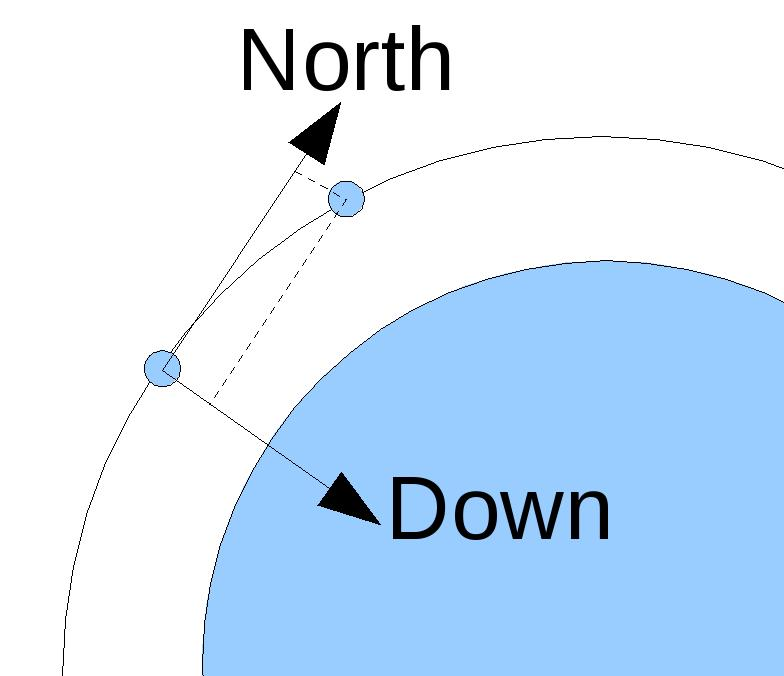
\includegraphics[width=2.5in]{figures/rectilinear.jpg}
\caption{The effect of the curvature of an orbit on the relative state using rectilinear coordinates.}
\label{fig:nedrectilinear}
\end{center}
\end{figure}












